\documentclass[twoside, final, 11pt]{articleMine}
\usepackage[english]{babel} \usepackage{a4wide}
\usepackage{amsmath,amssymb,accents} \usepackage{epsfig}
\usepackage{subfigure} \usepackage{units} \usepackage{graphicx}
\usepackage[displaymath, mathlines, right]{lineno} \usepackage{xspace}
\usepackage{color} \usepackage{epic,eepic,pstricks}
\usepackage{acronym} \usepackage{wrapfig,multicol}
\usepackage{deluxetable} \usepackage{todonotes} 
\usepackage{hyperref}
%\usepackage{slashbox}
\usepackage{lmodern} 
%\usepackage{caption}
\linenumbers
%\usepackage{showlabels}
\usepackage[draft]{showkeys}

%\usepackage[nolists, tablesfirst]{endfloat}
\graphicspath{{plots/}}
\newcommand*\patchAmsMathEnvironmentForLineno[1]{%
  \expandafter\let\csname old#1\expandafter\endcsname\csname #1\endcsname
  \expandafter\let\csname oldend#1\expandafter\endcsname\csname end#1\endcsname
  \renewenvironment{#1}%
     {\linenomath\csname old#1\endcsname}%
     {\csname oldend#1\endcsname\endlinenomath}}%
\newcommand*\patchBothAmsMathEnvironmentsForLineno[1]{%
  \patchAmsMathEnvironmentForLineno{#1}%
  \patchAmsMathEnvironmentForLineno{#1*}}%
\AtBeginDocument{%
\patchBothAmsMathEnvironmentsForLineno{equation}%
\patchBothAmsMathEnvironmentsForLineno{align}%
\patchBothAmsMathEnvironmentsForLineno{flalign}%
\patchBothAmsMathEnvironmentsForLineno{alignat}%
\patchBothAmsMathEnvironmentsForLineno{gather}%
\patchBothAmsMathEnvironmentsForLineno{multline}%
}
%\AtBeginFigures{\cleardoublepage}
%%%%%\parindent 5pt  
\parskip 1.2pt           % sets spacing between paragraphs
\def\Offline{\mbox{$\overline{\rm
Off}$\hspace{.05em}\raisebox{.4ex}{$\underline{\rm line}$}}\xspace}
\def\OfflineB{\mbox{$\bf\overline{\rm\bf
Off}$\hspace{.05em}\raisebox{.4ex}{$\bf\underline{\rm\bf line}$}}\xspace}

\def\eq#1{\begin{equation}#1\end{equation}}
%\def\al#1{\begin{align}#1\end{align}}
%\def\vc#1{{\bf #1}}
\def\pt#1{\accentset{\rightharpoonup}{#1}}
\include{myabbr}

\newcommand{\HRule}{\rule{\linewidth}{0.5mm}}
\newcommand{\VEM}{\mbox{VEM}}
\newcommand{\m}{\mbox{m}}

\let\stdsection\section  
%\renewcommand\section{\newpage\stdsection}  
 
\begin{document}

%\setpagewiselinenumbers
\modulolinenumbers[2]

%\linenumbers


\renewcommand\linenumberfont{\small\rmfamily}
\begin{center}
  \vspace*{-13ex}

  \rule{\linewidth}{0.1mm}  \\[17mm] {\huge  Helix detector status: May 2016}
     \begin{flushright}
       \small 
     
     \end{flushright}

  % 
\end{center}
% 
\vspace*{2ex} 
%
\thispagestyle{empty}
\noindent
\begin{abstract}
  \noindent
This note  presents the status of  the helix detectors. At  the end of
May  2016 they  were all  removed  from the  field and  tested in  the
assembly building  lab.  We present  the status in terms  of mechanics
and electronics.
\end{abstract}

%
\thispagestyle{empty}
%$\;$
%\listoftodos
%\newpage
\noindent
\section{Introduction}
The  helix  detectors  were   installed  at  the  beginning  of  March
2015. Since  then some problems arose  and among the  7 installed only
one seems to work properly. We removed the 7 detectors from the field,
and   tested   some   parts   of   them   in   lab.\\   We   give   in
table~\ref{tab:detref}  the correspondence  between station  name, LNA
serial number, antenna number and electronics box number.
\begin{table}[h!]
  \centering
  \caption{correspondence table between detector numbers}
  \label{tab:detref}
  \begin{tabular}{|c||c|c|c|c|c|c|c|}
    \hline
    station & Gilda  & Santy &  Jorge & Nono & Gringa & Eva & Rula \\
    \hline
    elec box number  & 11  & 10 & 09 & 08 & 05 & 03 & 02 \\
    \hline
    antenna number & 07 & 01 & 04 & 08 & 05 & 03 & 02 \\
    \hline
    LNA serial number & 022970 & 023232 & 023231 & 023230 & 022968 & 022967 & 022969\\
    \hline
  \end{tabular}
\end{table}




\section{Mechanics}
This first part reports on the state of the detectors as we found them
when we removed  them from the field.\\ All of  the antennas had their
metallic   cone  at   least   partly  distorted.    Pictures  in   the
figure~\ref{fig:cone}  show two  extreme cases:  Nono  detector's cone
(shown on  the left) is  distorted, in the  case of Eva (shown  on the
right) the  cone is no longer  attached to the  electronics box.\\ All
the antennas are in a similar state. The mechanics has to be improved.
\begin{figure}[!ht]
  \centering
  \hspace*{-3ex}
  \subfigure{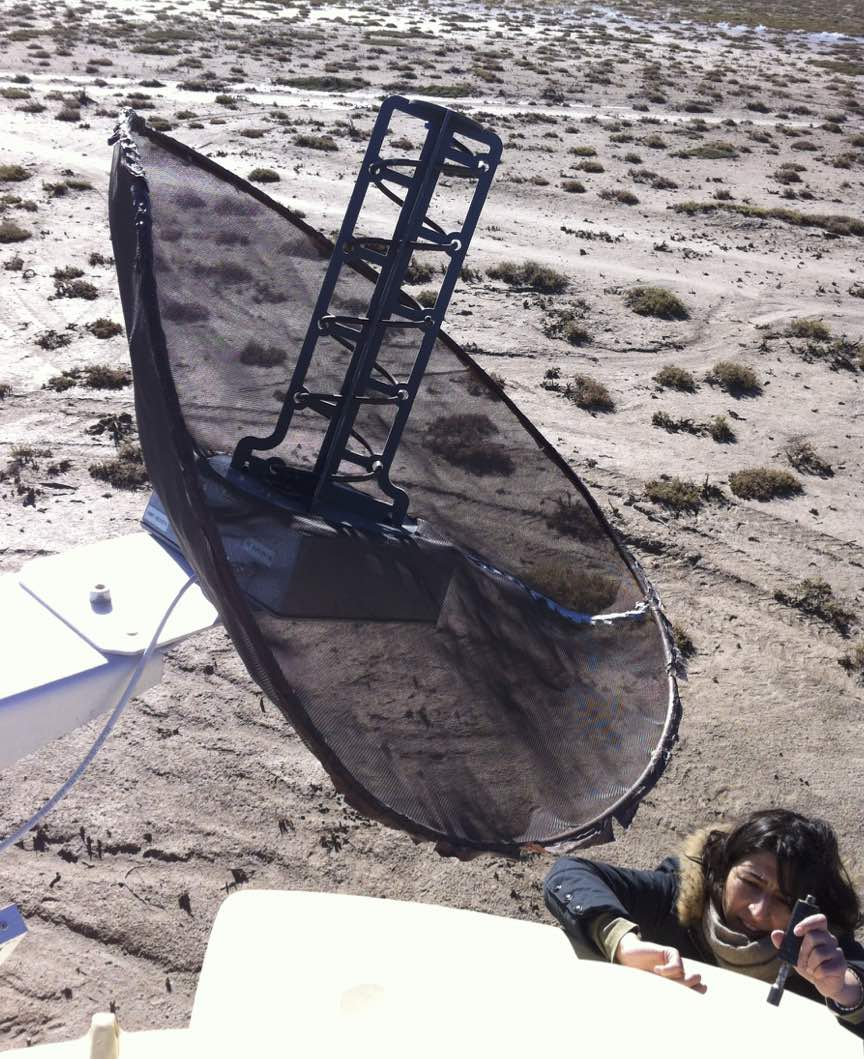
\includegraphics[width=0.49\linewidth]{nono.jpg}}
  \subfigure{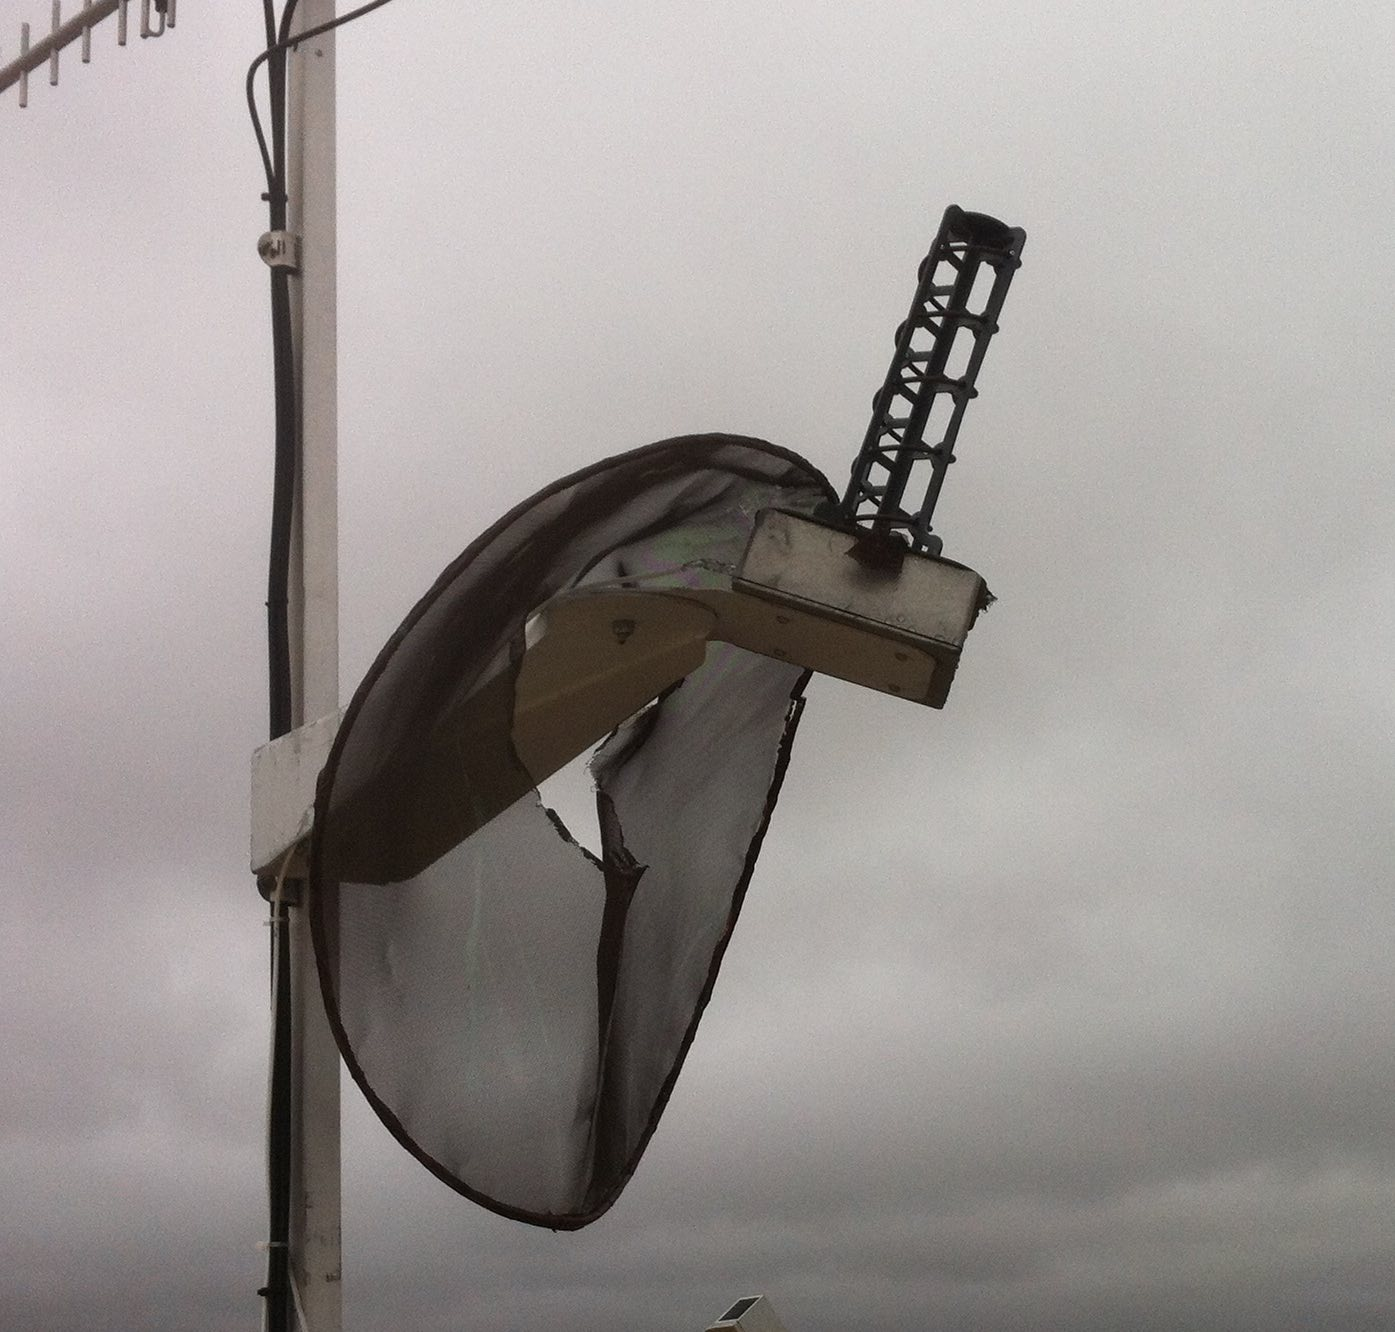
\includegraphics[width=0.49\linewidth]{eva.jpg}}
  \caption{Left:Nono, Right: Eva}
  \label{fig:cone}
\end{figure}

The second  problem encountered was  that water flooded inside  all of
the LNA boxes.   Water went inside the box through the  hole on top of
the box (see figure~\ref{fig:lnabox}  left).  Some boxes had still 1-2
cm  of  water  in  them  and  rust started  to  grow  inside  the  box
(figure~\ref{fig:lnabox} right).

\begin{figure}[!ht]
  \centering
  \hspace*{-3ex}
  \subfigure{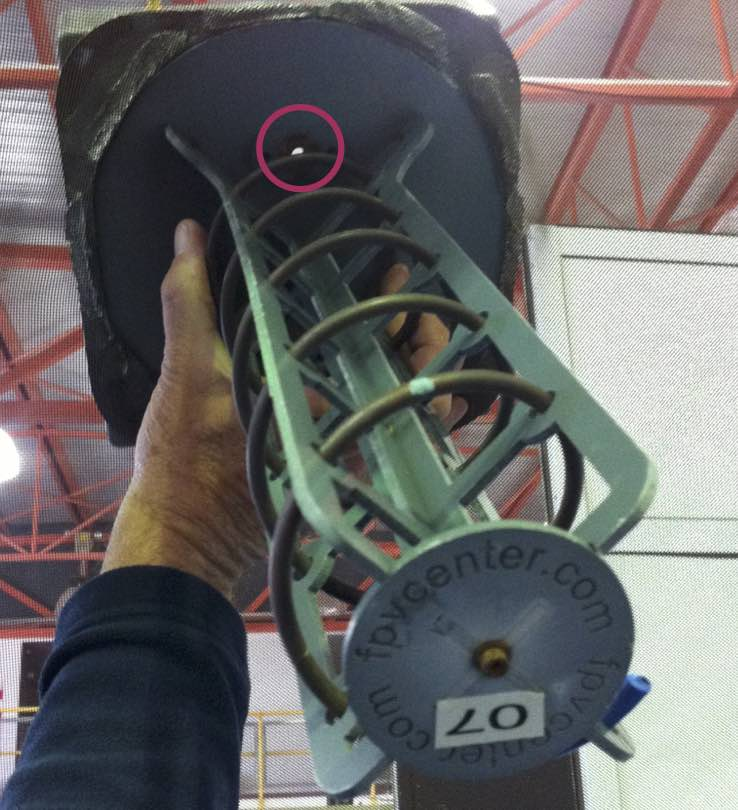
\includegraphics[width=0.49\linewidth]{boitehelix2.jpg}}
  \subfigure{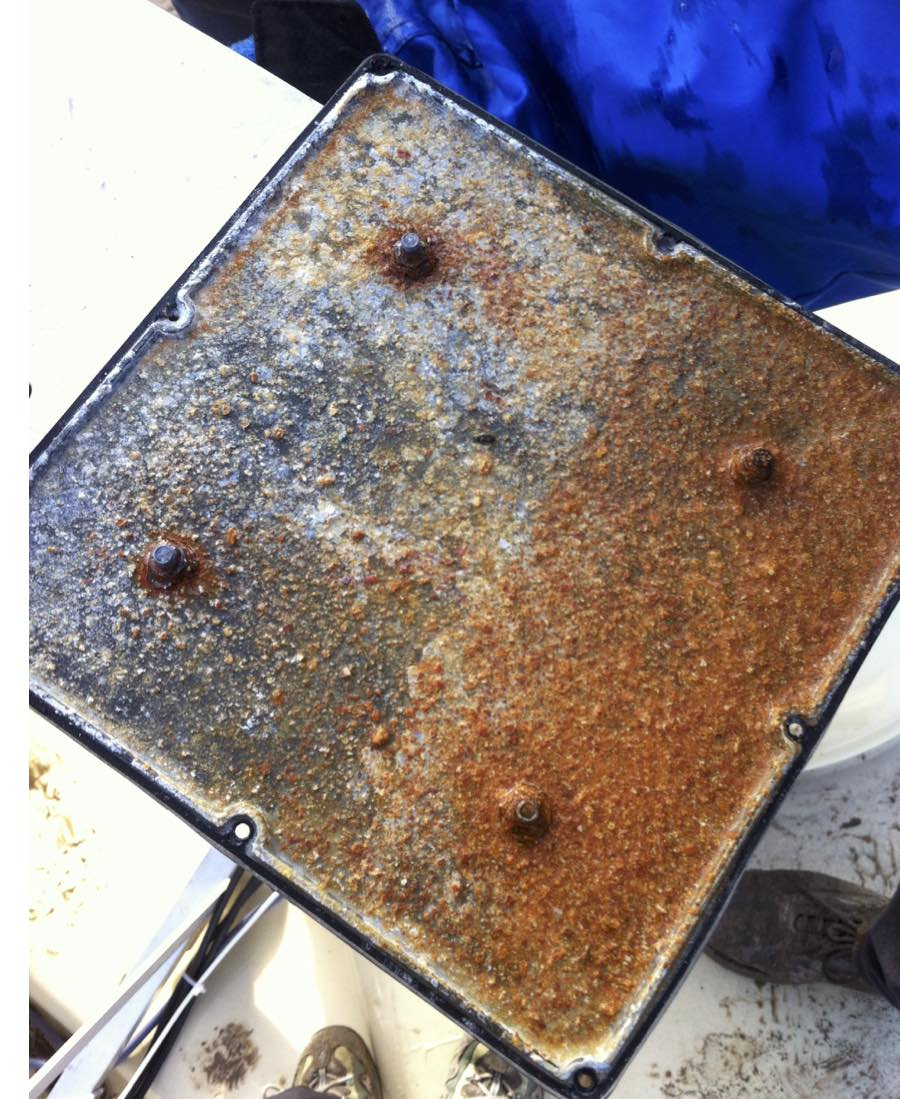
\includegraphics[width=0.49\linewidth]{boxsanty.jpg}}
  \caption{Left: helix antenna, circled the hole where water went into
    the LNA box. Right: rust in Santy's LNA box}
  \label{fig:lnabox}
\end{figure}




\section{Antenna and LNA}
Here we  show the  characteristics of  the RF parts.   We show  in the
figure~\ref{fig:vswrant} the VSWR of the antennas. Jacques identified a
bad contact  on the antenna FPV01.   All of the other  antennas have a
low  VSWR (close  to 1  in our
frequency bandwidth as we  expect for  an impedance  match).
\begin{figure}[!ht]
  \centering
  \hspace*{-3ex}
  \subfigure{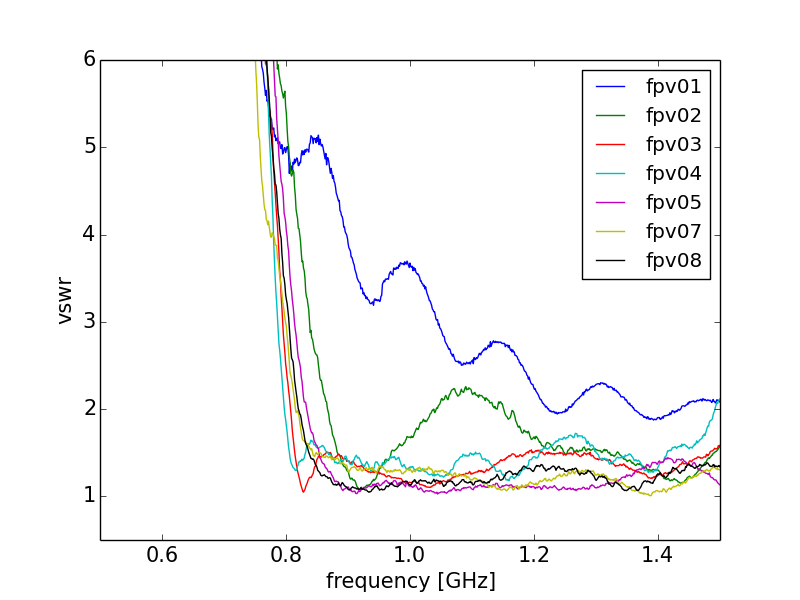
\includegraphics[width=0.60\linewidth]{s11_ant.png}}
  \caption{antenna VSWR, measured in lab}
  \label{fig:vswrant}
\end{figure}

The characteristics  of the LNA were  also measured: the  VSWR and the
gain are shown in the figure~\ref{fig:lnas11} and ~\ref{fig:lnas21}.

\begin{figure}[!ht]
  \centering
  \hspace*{-3ex}
  \subfigure{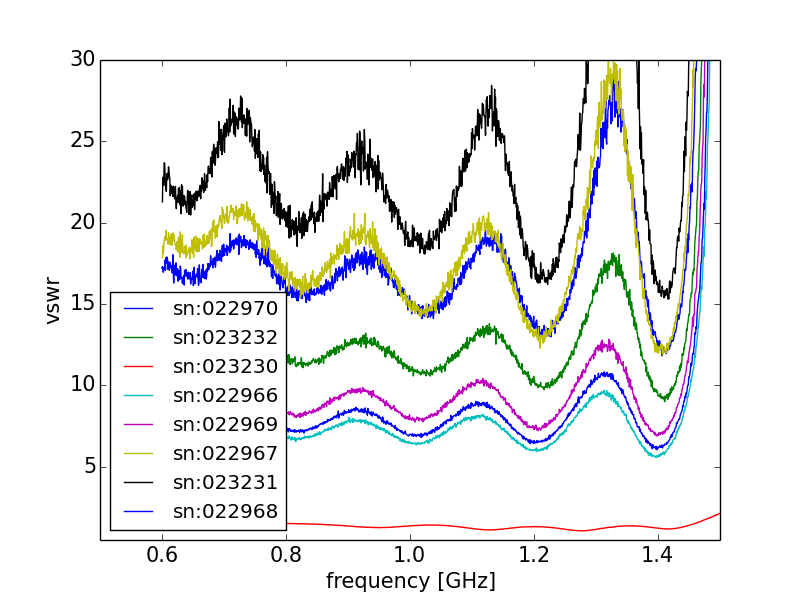
\includegraphics[width=0.60\linewidth]{s11_LNA2.png}}
  \caption{LNA VSWR}
  \label{fig:lnas11}
\end{figure}
\begin{figure}[!ht]
  \centering
  \hspace*{-3ex}
  \subfigure{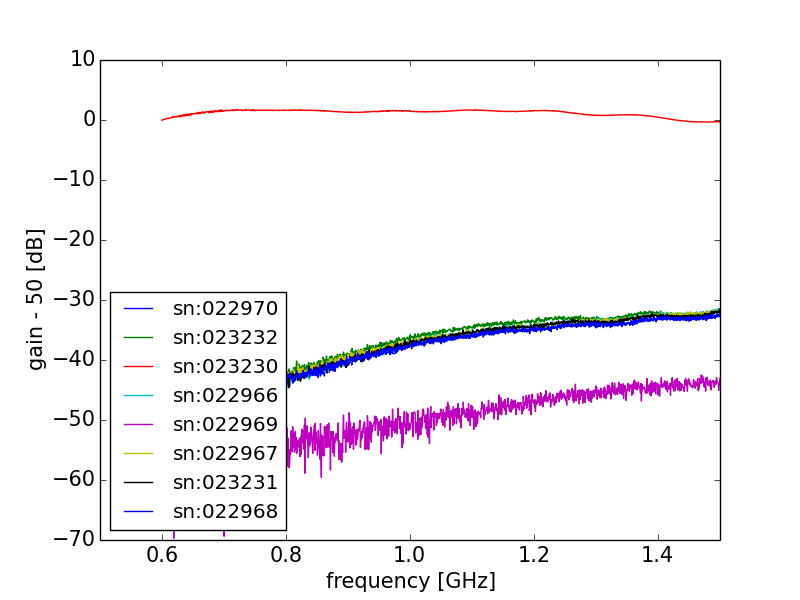
\includegraphics[width=0.60\linewidth]{gain_LNA2.png}}
  \caption{LNA gain. The measurement of the gain was done with a 50dB attenuator.}
  \label{fig:lnas21}
\end{figure}

On the figure \ref{fig:lnas21} it is  clear that only one LNA is still
working, the sn023230, that is the  one that was installed on Nono. It
has the expected gain (50dB) and a low VSWR.  All of the other ones are
broken and almost all have the same characteristics.  \\ So the LNA is
the main failure of the system.  The LNAs broke for an unknown reason.
Possible sources of failure are:
\begin{itemize}
\item a power  surge at the LNA input (for  instance an electro static
  discharge or an over voltage due to a thunderstorm)
\item the humid/water environment (for instance if the LNA was flooded
  inside the box)
\end{itemize}

A  possible  solution  to  the  power  surge could  be  to  install  a
transformer (with coil), or a diode  system before the LNA. We need to
evaluate the effect  of these devices on the  noise figure (since they
need to be placed before the LNA).

\section{electronic box}
The  last part  of  the detector  is  the electronic  box.  They  were
installed under the  SD electronics dome, and they  were found in good
shape. None of them suffered from an obvious problem.\\ We tested them
with the setup shown in the figure~\ref{fig:setupbox}. 
\begin{figure}[!ht]
  \centering
  \hspace*{-3ex}
  \subfigure{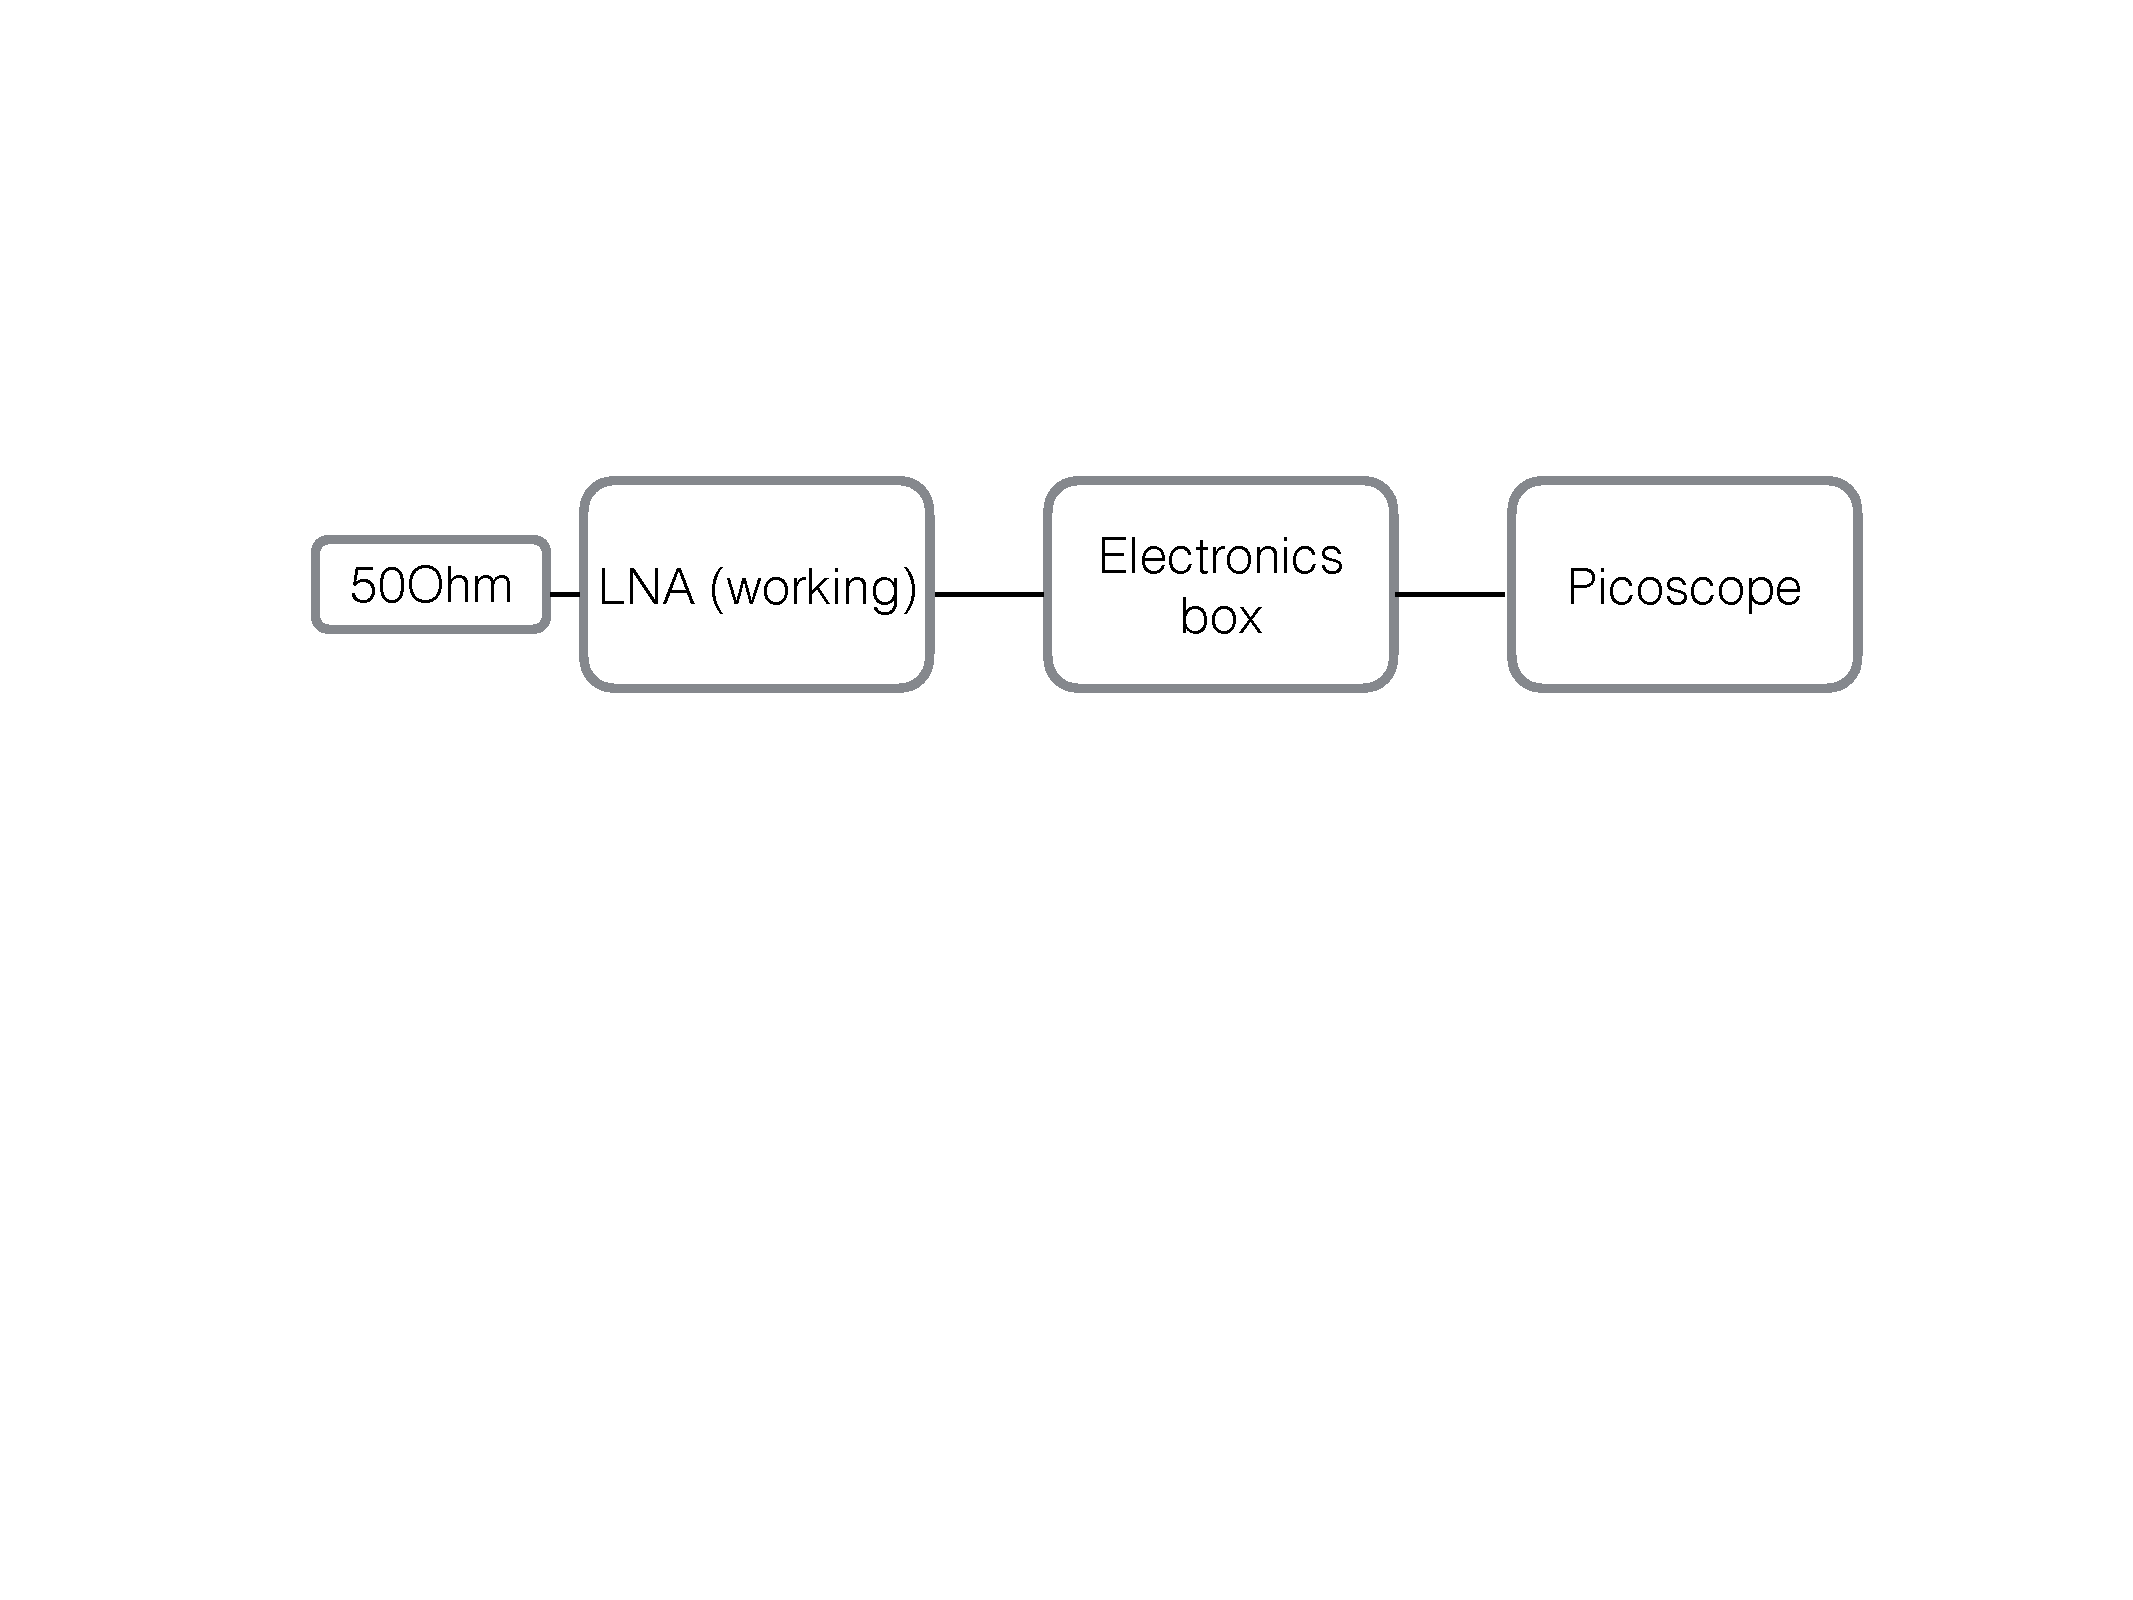
\includegraphics[width=0.60\linewidth]{setupbox.pdf}}
  \caption{setup to evaluate  the electronics box characteristics. The
    LNA and the  load are installed in a LNA box  with an antenna over
    it, but the antenna is NOT connected.}
  \label{fig:setupbox}
\end{figure}
This setup allows us to compare all the boxes with the same reference,
i.e. 300K of  the 50Ohm load. We acquire data  (10 waveforms) with the
Picosope  (4MS/s,  2ms/div)  for  each  box.  The  mean  and  standard
deviation  are  reported  in the  table~\ref{tab:boxtab}.   (reminder:
after the box 100mV=1dB)
\begin{table}[h!]
  \centering
  \caption{average and RMS measurement of the electronics boxes}
  \label{tab:boxtab}
  \begin{tabular}{|c||c|c|c|c|c|c|c|c|c|}
    \hline
    box number & 11  & 10 & 09 & 08 & 05 & 04 & 03 & 02 & 06 \\
    \hline
    station & Gilda  & Santy &  Jorge & Nono & Gringa & - & Eva & Rula & -  \\
    \hline
    average (baseline)[mV] & -469 & -291 &  -270 & -477 & -305 & -548 & -450 & -445 & -774 \\
    \hline
    standard dev  [mV] & 47 & 97 & 40 & 86 & 52 & 83 & 58 & 43 & 50 \\
    \hline
  \end{tabular}
\end{table}
\\
\textbf{notes at data taking}
\begin{itemize}
\item box 09: baseline varies with time ($\simeq$ 1mV/min)
\item box 08: remeasured at $ average = -438 mV$ and $\sigma = 60 mV$
\item box 04: has peaks every 10ms
\item box 03: baseline varies with time ($\simeq$ 1.5mV/min)
\item box 02: baseline varies with time (from -430 to -443 in the first minute, -445 after two minutes)
\item box 06: has peaks every 10ms
\end{itemize}

\paragraph{remarks}
\begin{enumerate}
\item  One can see  that the  baselines are  quite different,  this of
  course   depends   on   how   much  was   rotated   the   adjustable
  resistor. However when  we look at the installation  sheet, for four
  detectors (Gilda, Santy, Eva, and Rula) the baseline was not changed
  at the installation, that means  we can directly compare the average
  values  in the table~\ref{tab:boxtab}.   We see  that Eva,  Rula and
  Gilda differ  by less  than 0.2dB, but  Santy's baseline  differs by
  around 150 mV (1.5dB).
\item A second  remark is about the RMS, one  can see two populations:
  one around 50mV and one around 90mV. This is strange because the RMS
  should not depend on the  adjustable resistor settings, it should be
  approximately the  same for all the  boxes because the  input is the
  same. This problem has to  be investigated because the RMS should be
  a direct measurement of the input noise, so a difference of a factor
  2 is worrying.
\item  Two boxes  (number 4  and number  6) showed  peaks with  a 10ms
  period  (cf fig~\ref{fig:peaks}).   We still  don't know  where this
  noise comes from.  We sometimes  saw it and then it disappeared, its
  amplitude was also changed by the orientation of the box (containing
  the  LNA  and the  50Ohm  load). It  could  be  an anthropic  signal
  captured  by the  antenna  or some  part  of the  box (the  assembly
  building is very noisy at these frequencies).
  \begin{figure}[!ht]
    \centering
    \hspace*{-3ex}
    \subfigure{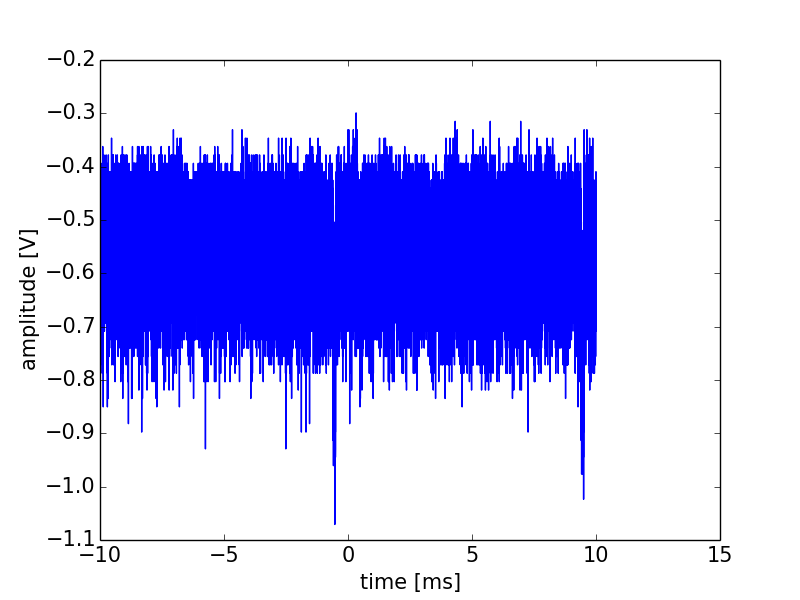
\includegraphics[width=0.49\linewidth]{peaks.png}}
    \subfigure{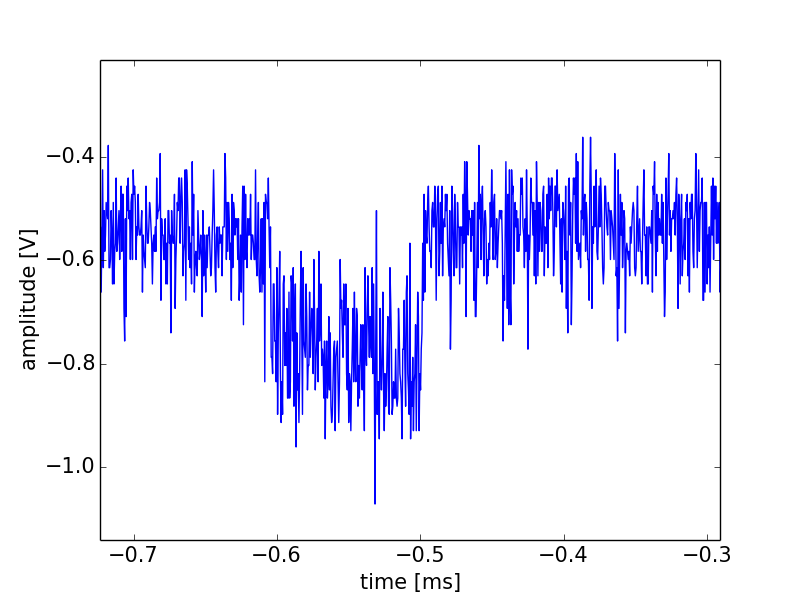
\includegraphics[width=0.49\linewidth]{peaks2.png}}
    \caption{example of trace of the box 4 (left) and zoomed (right)}
    \label{fig:peaks}
  \end{figure}
\item As for the time varying baseline, this could be explained by the
  warm up time  of the electronics.  Mari did  a longer measurement of
  box9.  The results are  plotted in the fig~\ref{fig:box9vstime}, the
  baseline drops by a few tens of mV in 30 minutes.  The decrease rate
  gets smaller with time (the derivative gets close to zero).
  \begin{figure}[!ht]
    \centering
    \hspace*{-3ex}
    \subfigure{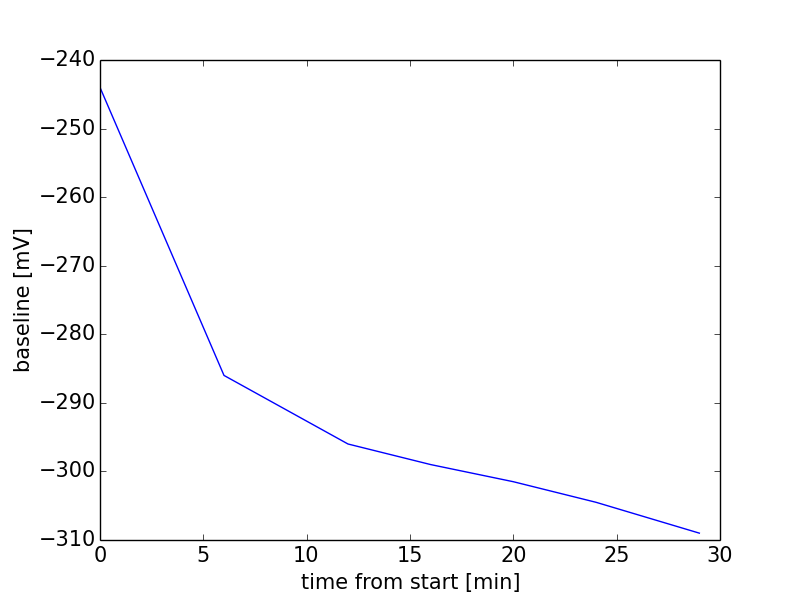
\includegraphics[width=0.49\linewidth]{box9vstime.png}}
    \caption{baseline versus time for the box number 9}
    \label{fig:box9vstime}
  \end{figure}
\end{enumerate}

\section*{conclusion}
We  have  gone  through  the  different step  to  simulate  an  EASIER
waveform.  In  particular, we  have detailed the  generation of  an RF
waveform from a realistic spectrum. We also improved the simulation of
the  adaptation  electronics. The  full  simulation  is then  compared
against  data looking at  the traces  fluctuation in  ADC.  We  find a
simulated waveform overestimated the  fluctuation by a small number of
ADC.

\addcontentsline{toc}{chapter}{Bibliography}                                 
\bibliographystyle{atlasnote}
\bibliography{easier}
%% \newpage
%% \begin{thebibliography}{9}
%% \bibitem{gorham}P. W. Gorham et al., Phys. Rev. D 78, 032007 (2008).
%%   [arXiv:0705.2589 [astro-ph]]
%% \bibitem{augerpolar} The Pierre Auger Collaboration, Phys. Rev. D 89, 052002 (2014)
%% \bibitem{crome}
%% \end{thebibliography}

\end{document}
